\documentclass[12pt]{article}

\usepackage{sbc-template}
\usepackage{graphicx,url}
\usepackage[utf8]{inputenc}
\usepackage[brazil]{babel}
\usepackage{amsmath}
% \usepackage[latin1]{inputenc}  

\sloppy

\title{Trabalho Final \\ Computação Reconfigurável}

\author{Bruno Feitosa\inst{1}}

\address{Instituto de Ciências Matemáticas e de Computação -- Universidade de São Paulo
\email{feitosa.bruno@usp.br}
}

\begin{document} 

\maketitle

\begin{abstract}
This paper implements and discuss a HDL example of a single layer of a
Convolution Neural Network, and compares its performance to a equivalent Javascript
implementation of the same CNN Layer.

\end{abstract}
     
\begin{resumo} 
Este artigo implementa e discute um exemplo em HDL para uma única camada de uma
Rede Neural Convolucional, e compara sua performance em relação a uma implementação equivalente
em Javascript da mesma camada CNN.

\end{resumo}

\nocite{GNU:MP,GNU:MPFR}

\section{Arquitetura}

A arquitetura implementada pode ser vista na Figura \ref{fig:arch_base} a seguir.
A arquitetura consiste de um Controlador de Endereçamento, um bloco de acesso à Imagem,
um bloco de acesso ao Filtro, e um Neurônio.\\

\begin{figure}[h]
	\centering
	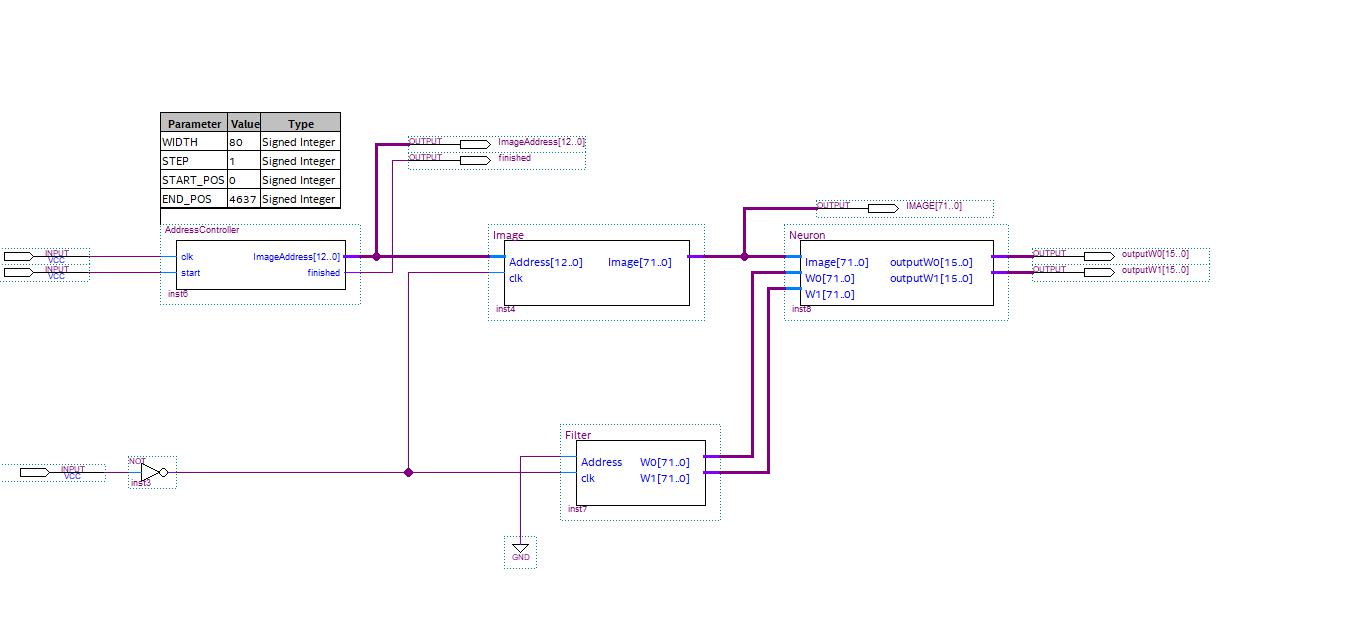
\includegraphics[width=.8\textwidth]{CNN_Layer.jpg}
	\caption{Arquitetura de uma Camada CNN}
	\label{fig:arch_base}
\end{figure}

A implementação com paralelização de Neurônios usou 4 Neurônios, e pode ser vista na Figura
\ref{fig:arch_par}.\\

\begin{figure}[h]
	\centering
	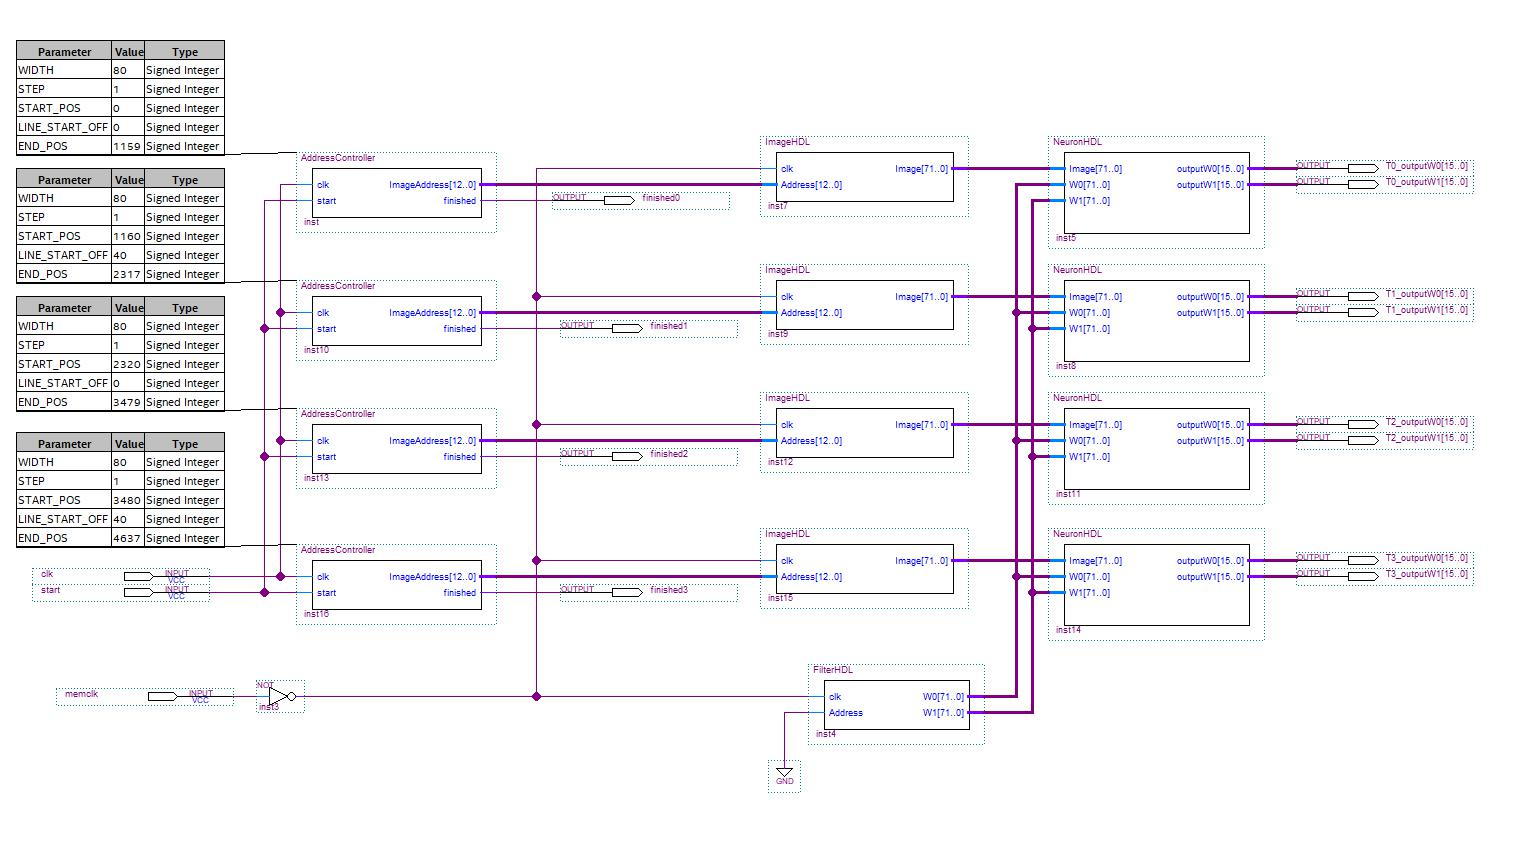
\includegraphics[width=.8\textwidth]{CNN_Layer-P.jpg}
	\caption{Arquitetura de uma Camada CNN com Paralelização}
	\label{fig:arch_par}
\end{figure}

O projeto e simulação da implementação foram feitas na placa 5CGXFC7C7F23C8, usando a FPGA
Cyclone V.\\

\subsection{Controlador de Endereçamento}

A figura onde a rede é aplicada possui um tamanho de 80x60 pixels, onde cada pixel é guardado
em 1 byte (8 bits). Isso implica que o Controlador de Endereço deve gerar endereços de 0 até
4779. O Filtro é aplicado em cada bloco de 3x3 pixels, e esta aplicação em particular
utiliza um bloco de 3x3 pixels a cada ciclo de clock.\\
Cada bloco de 3x3 pixels é selecionado com base no primeiro pixel no topo esquerdo do bloco.
Isso implica que o controlador de endereços gera endereços de 0 até 2 pixels antes do final
da linha, e não gera endereços para as duas últimas linhas. Dessa forma, o Controlador de
Endereços gera um total de $4524$ ($(80-2).(60-2)$) endereços.\\

\subsection{Bloco de Acesso a Imagem}

Para cada endereço de referência recebido pelo Controlador de Endereçamento, o bloco de acesso
a Imagem acessa em paralelo os 9 pixels do bloco de 3x3 pixels no qual o filtro será aplicado.
A implementação pode ser vista na Figura \ref{fig:image_block} a seguir. Cada Byte é acessado independentemente em uma cópia da imagem, guardada em uma ROM.\\

\begin{figure}[h]
	\centering
	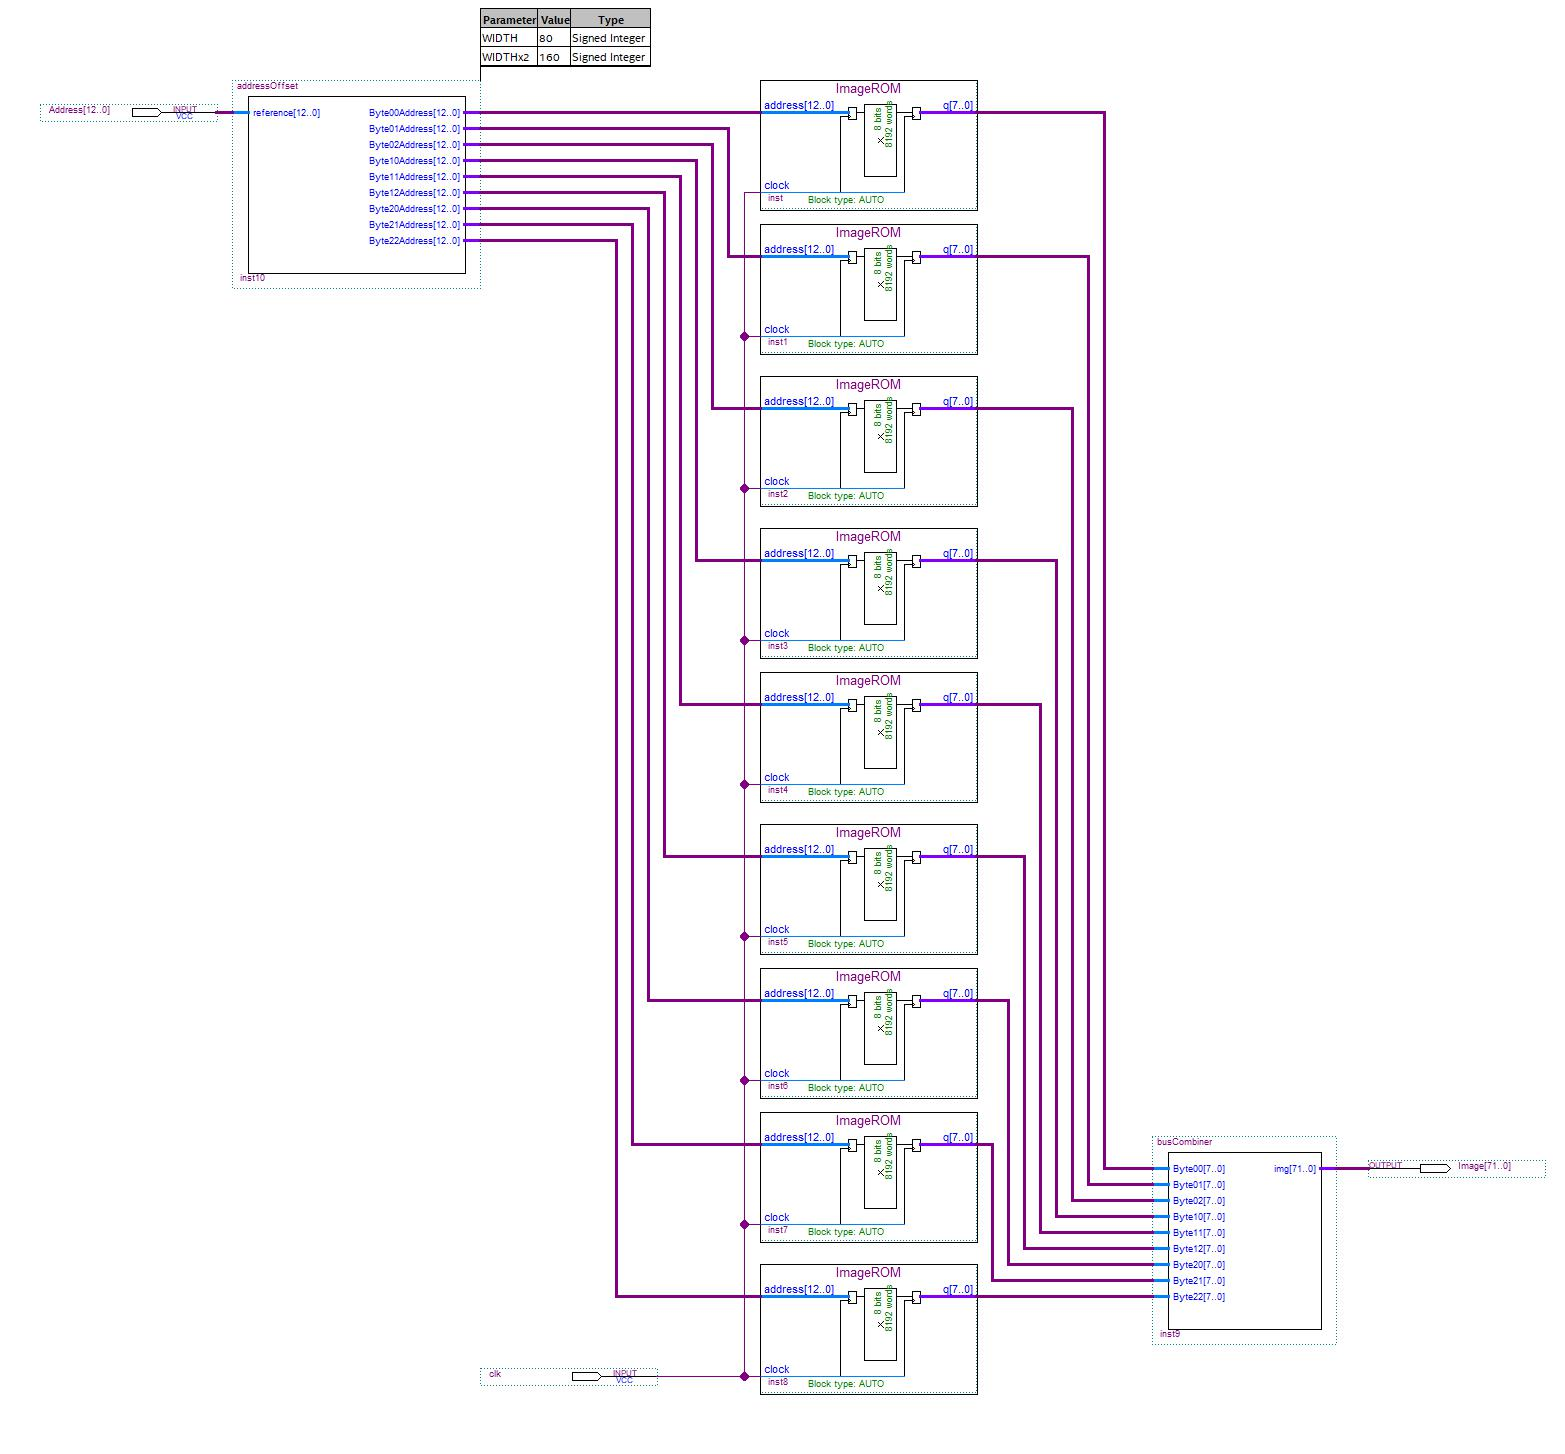
\includegraphics[width=.8\textwidth]{CNN_Layer-Image.jpg}
	\caption{Bloco de Acesso a Imagem}
	\label{fig:image_block}
\end{figure}

O Byte00 tem endereço igual ao de referência, o Byte01 tem um offset de uma unidade em relação
a referência, o Byte02 tem duas unidades de offset em relação a referência,
o Byte10 tem um offset igual a largura da imagem em relação ao endereço de referência,
o Byte11 tem um offset igual a largura da imagem mais uma unidade em relação a referência,
o Byte12 tem um offset igual a largura da imagem mais duas unidade em relação a referência,
o Byte20 tem um offset igual duas vezes a largura da imagem em relação a referência,
o Byte21 tem um offset igual duas vezes a largura da imagem mais uma unidade, e
o Byte22 tem um offset igual duas vezes a largura da imagem mais duas unidades.\\

Todos os bytes são concatenados em um vetor de 72 bits (9 bytes), que é passado para o Neurônio.

\subsection{Bloco de Acesso ao Filtro}

Cada um dos dois Filtros está implementado em uma ROM. Cada Filtro é acessado diretamente,
todos os 9 valores sendo passados para o Neurônio. Os Filtros são consituídos de 9 posições
com valores de tamanho de um byte. Os valores são valores inteiros com sinal.\\

\subsection{Neurônio}

O Neurônio é implementado em lógica combinacional, calculando o valor resultante do filtro
em cada bloco de 3x3 pixels assim que disponibilizados pelo Endereçador e Imagem.
Todos os valores do byte da Imagem e do Filtro são mantidos em inteiros com sinal. Como o valor
do byte não possui sinal, um bit zerado é adicionado a palavra da imagem. Dessa forma,
a sintetização trata a multiplicação do filtro pela imagem como uma multiplicação de valores
com sinal.\\

Como os valores do filtro e da imagem tem tamanho de um byte, o resultado da multiplicação tem
tamanho máximo de 2 bytes. O valor resultante ainda poderia ser ajustado por um peso equilibrando
a soma dos 9 blocos (divisão por 9), mas isto poderia ser feito também na função de ativação,
ou mantido e levado em conta na aplicação das camadas seguintes.\\

\section{Notas sobre a Arquitetura}

O Endereçador e a Imagem são alimentados pelo mesmo clock. Porém, o clock da Imagem é atrasado
por meio ciclo de clock por meio de uma porta de negação (NOT) em relação ao endereçador.
Isso facilita a sincronização entre a disponibilização do endereço para a ROM e a solicitação
do valor guardado no endereço, incluindo um atraso de meio ciclo na saída do resultado em
relação ao clock do endereçamento.\\

Apesar disso, foi necessário separar as fontes de clock para que os cálculo de timing do
Quartus não resultassem em um valor muito baixo de frequência máxima de operação (cerca de 
60 MHz). Quando testados isoladamente, os blocos de acesso a ROM tinham frequência
máxima de operação entre 250 MHz e 300 MHz, enquanto os blocos de endereçamento tinham
frequência máxima de cerca de 240 MHz. Após o isolamento dos clocks e declaração de 
caminhos falsos entre os clocks de memória e endereçamento, a compilação do projeto demonstrou
os clocks de endereçamento e memória com seus valores próximos dos testados isoladamente.\\

A implementação paralela utiliza 4 Neurônios em paralelo, onde cada Neurônio processa
um quarto da imagem. Para facilitar a visualização da implementação e não gerar novos
componentes no Quartus, cada Neurônio possui uma cópia completa da Imagem. O recurso crítico
desta implementação foram os DSPs disponíveis no Cyclone V, onde cada Neurônio utiliza 6 DSPs
($10\%$ dos 156 disponíveis), enquanto também gastavam $5\%$ dos blocos de memória, o
que reduziu a preocupação de reduzir o consumo de memória.\\

\section{Resultados e Discussões}

Os recursos utilizados e tempo necessário para execução do filtro podem ser vistos
na Tabela \ref{tab:comp} a seguir para as implementações com 1 e 4 Neurônios.
Ambas aplicações foram simuladas e compiladas com frequência de 200 MHz.\\

\begin{table}[h]
	\centering
	\caption{Comparação de Performance Entre 1 e 4 Neurônios}
	\begin{tabular}{|l|c|c|r|}
		\hline
		 & 1 Neurônio & 4 Neurônios & Recurso Disponível \\
		\hline
		Frequência Máxima (end)		& 250,06 MHz	& 244,38 MHz	& - \\
		Frequência Máxima (mem)		& 240,04 MHz	& 240,04 MHz	& - \\
		ALMs 						& 75			& 307			& 56.480 \\
		Registradores				& 21			& 84			& - \\
		Blocos de Memória (bits)	& 345.744		& 1.382.544		& 7.024.640 \\
		DSP							& 16			& 64			& 156 \\
		Setup Slack (end)			& 1,001 ns		& 0,908	ns		& - \\
		Setup Slack (mem)			& 2,323 ns		& 2,323 ns		& - \\
		Hold Slack (end)			& 0,547 ns		& 0,482 ns		& - \\
		Hold Slack (mem)			& 0,925 ns		& 0,925 ns		& - \\
		Timing (Slack em pior caso)	& 1,001 ns		& 0,908 ns		& - \\
		Tempo de Execução			& 22,6 $\mu$s	& 5,7 $\mu$s	& - \\
		\hline
	\end{tabular}
	\label{tab:comp}
\end{table}
	
Para comparação, foi aplicado o mesmo algoritmo em na mesma imagem, porém executado em linguagem
Javascript, de forma completamente sequencial. O algoritmo foi executado 1000 vezes, e os
valores mínimos, máximos, e médios foram registrados. Devido ao código estar sendo executado
em um computador rodando um sistema operacional, os valores máximos são de algumas execuções
ficam muito fora da faixa de valores médios, devido ao sistema operaçional parar a execução
do algoritmo para realizar outras operações. Para melhor observar o tempo de execução, foram
filtrados os valores máximo e mínimo dos 1000 testes executados duas vezes seguidas.
Os valores máximos, mínimos e médios podem ser observados na Tabela \ref{tab:comp_to_sequ}
a seguir.\\

\begin{table}[h]
	\centering
	\caption{Tempo de Execução do Filtro em Javascript}
	\begin{tabular}{|l|c|c|c|r|}
		\hline
		Execução	& Máximo	& Mínimo	& Médio		& Número de Execuções \\
		\hline
		Original	& 41,220 ms	& 0,285 ms	& 0,417 ms	& 1.000 \\
		1º Filtro	& 12,365 ms	& 0,285 ms	& 0,378 ms	& 991 \\
		2º Filtro	& 1,655 ms	& 0,290 ms	& 0,366 ms	& 985 \\
		\hline
	\end{tabular}
	\label{tab:comp_to_sequ}
\end{table}

O processador do computador onde estes testes foram feitos é um Intel Core i5-5200U @ 2.70GHz,
com dois núcleos de processamento. A execução sequencial não foi paralelizada.\\

\section{Conclusões}

A execução do filtro em uma FPGA criou um hardware especializado para a aplicação do Filtro CNN,
com capacidade de execução muito superior a execução sequencial em um processador comum.\\

Operações matriciais também podem ser aceleradas por GPUs. Porém, FPGAs ainda possuem uma maior
flexibilidade e capacidade de especialização.

\end{document}
